\section{Discrete manifolds}
We will remind ourselves of the definition of a classical simplicial complex, in sets. Then we will create a higher type from the data of a complex, using pushouts. The type will both imitate the structure of the set-based complex and will contain explicit maps into it from the sets of the complex.

\subsection{Abstract simplicial complexes}

\begin{mydef}
An \defemph{abstract simplicial complex \( M\defeq[M_0,\ldots,M_n] \) of dimension \( n \)} is an ordered list consisting of a set \( M_0 \) of vertices, and for each \( 0<k\leq n \) a set \( M_k \) of subsets of \( M_0 \) of cardinality \( k+1 \), such that any \( (j+1) \)-element subset of \( M_k \) is an element of \( M_j \). The elements of \( M_k \) are called \defemph{\( k \)-faces}. Denote by \( \simcomp \) the type of abstract simplicial complexes of dimension \( n \) (where the suffix \( \mathsf{Set} \) reminds us that this is a type of sets). Let \( M_{\leq k}= [M_0,\ldots,M_k] \) and note that \( M_{\leq n}=M \). We call \( M_{\leq k} \) the \defemph{\( k \)-skeleton} of \( M \), and it is a (\( k \)-)complex in its own right. \( M \) is automatically equipped with a chain of inclusions of the skeleta \( M_0\hookrightarrow M_{\leq 1}\hookrightarrow\cdots\hookrightarrow M_{\leq n}=M \). 
\end{mydef}


\begin{mydef}
Let \( \Delta^n \) be the standard \( n \)-simplex in \( \rr^n \) given by \( \{x_1,\ldots,x_n|\sum_i x_i\leq 1\} \). Let \( M:\simcomp \). The \defemph{geometric realization} \( |M|:\Topcat \) of \( M \) in the category of topological spaces is given inductively as follows: \( |M_0|=M_0 \), and given \( |M_{\leq k-1}| \) we form \( |M_{\leq k}| \) by the pushout in sets
\end{mydef}
% https://q.uiver.app/#q=WzAsNCxbMSwxLCJ8TV97a318Il0sWzEsMCwifE1fe2stMX18Il0sWzAsMCwiTV97a31cXHRpbWVzXFxwYXJ0aWFsXFxEZWx0YV5rIl0sWzAsMSwiTV97a31cXHRpbWVzXFxEZWx0YV5rIl0sWzIsMSwiXFxtYXRocm17YXR0YWNofSJdLFsyLDMsIlxcbWF0aHJte2lkfVxcdGltZXNcXG1hdGhybXtpbmNsfSIsMix7InN0eWxlIjp7InRhaWwiOnsibmFtZSI6Imhvb2siLCJzaWRlIjoidG9wIn19fV0sWzMsMF0sWzEsMCwiaV9rIl0sWzAsMiwiIiwxLHsic3R5bGUiOnsibmFtZSI6ImNvcm5lci1pbnZlcnNlIn19XV0=
\begin{center}
\begin{tikzcd}
  {M_{k}\times\partial\Delta^k} & {|M_{\leq k-1}|} \\
  {M_{k}\times\Delta^k} & {|M_{\leq k}|}
  \arrow["{\mathrm{attach}}", from=1-1, to=1-2]
  \arrow["{\mathrm{id}\times\mathrm{incl}}"', hook, from=1-1, to=2-1]
  \arrow["{i_k}", from=1-2, to=2-2]
  \arrow[from=2-1, to=2-2]
  \arrow["\ulcorner"{anchor=center, pos=0.125, rotate=180}, draw=none, from=2-2, to=1-1]
\end{tikzcd}
\end{center}
which attaches each \( k \)-simplex by taking the convex hull of the appropriate \( k+1 \) points in \( |M_{\leq k-1}| \).
The collection of vertical maps on the right gives a sequence of inclusion maps of skeleta \( |M_0|\xrightarrow[]{i_1}|M_{\leq 1}|\xrightarrow[]{i_2}\cdots\xrightarrow[]{i_n}|M_{\leq n}|=|M| \).

\begin{mydef}
In an abstract simplicial complex \( M \) of dimension \( n \), the \defemph{link} of a vertex \( v \) is the \( n-1 \)-dimensional subcomplex containing every face \( m\in M_{n-1} \) such that \( v\notin m \) and \( m\cup v \) is an \( n \)-face of \( M \).
\label{def:link}
\end{mydef}

The link is easier to understand as all the neighboring vertices of \( v \) and the subcomplex containing these. See for example Figure~\ref{fig:link}.

\begin{figure}[h]
\centering
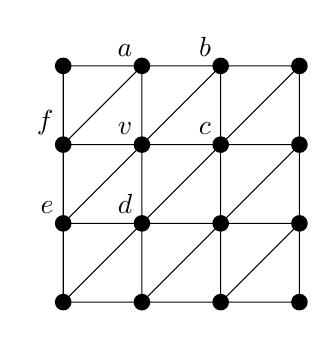
\begin{tikzpicture}
  \draw
    (0, 0) grid[step=1cm] (3, 3)
    (0, 2) -- (1, 3)
    (0, 1) -- (2, 3)
    (0, 0) -- (3, 3)
    (1, 0) -- (3, 2)
    (2, 0) -- (3, 1)
  ;
  \fill[radius=3pt]
    \foreach \x in {0, ..., 3} {
      \foreach \y in {0, ..., 3} {
        (\x, \y) circle[]
      }
    }
  ;
  \path[above left]
    \foreach \p/\v in {
      {1, 3}/a,
      {2, 3}/b,
      {0, 2}/f,
      {1, 2}/v,
      {2, 2}/c,
      {0, 1}/e,
      {1, 1}/d%
    } {
      (\p) node {$\v$}
    }
  ;
\end{tikzpicture}
\caption{The link of \( v \) in this complex consists of the vertices \( \{a,b,c,d,e,f\} \) and the edges \( \{ab,bc,cd,de,ef,fa\} \), forming a hexagon.}
\label{fig:link}
\end{figure}

\begin{mydef}
A \defemph{combinatorial manifold} (or \defemph{combinatorial triangulation}) of dimension \( n \) is a simplicial complex of dimension \( n \) such that the link of every vertex is a \defemph{simplicial sphere} of dimension \( n-1 \) (meaning its geometric realization is homeomorphic to an \( n-1 \)-sphere). Denote by \( \combmfdset \) the type of combinatorial manifolds of dimension \( n \) (which the notation again reminds us are sets).
\end{mydef}

In a 2-dimensional combinatorial manifold the link is a polygon. See Figure~\ref{fig:sphere_triangulation} for some examples of 2-dimensional combinatorial manifolds of genus 0, 1, and 3.

A classical 1940 result of Whitehead, building on Cairn, states that every smooth manifold admits a combinatorial triangulation\cite{whitehead_triangulation}. So it appears reasonably well motivated to study this class of objects. See for example the classic book by Kirby and Siebenmann\cite{kirby_siebenmann}. There are important examples in four dimensions of topological manifolds that do not have any smoothness structure or triangulation. These will be out of reach of the theory we are building.

\begin{figure}[h]
\centering
\includegraphics[width=100pt]{triangulated_sphere.pdf}
\includegraphics[width=100pt]{Torus-triang.png}
\includegraphics[width=100pt]{triangulated_genus3.pdf}
\caption{Combinatorial triangulations of a sphere, torus, and 3-holed torus. Sphere created with the tool \texttt{stripy}; torus from Wikipedia (\href{https://commons.wikimedia.org/w/index.php?curid=30856793}{By Ag2gaeh} - Own work, CC BY-SA 3.0.); 3-holed torus from Wikipedia (\href{https://commons.wikimedia.org/wiki/File:Tri-brezel.svg}{By Ag2gaeh} - Own work, CC BY-SA 3.0.)}
\label{fig:sphere_triangulation}
\end{figure}

\subsection{Higher inductive combinatorial manifolds}

Instead of \( |M|:\Topcat \) we can use the simplicial complex to obtain \( \mm:\Type \) by forming a sequence of \emph{homotopy} pushouts. For example in dimension 1 we could take the triangle with vertices \( \{v_1, v_2, v_3\} \) and edges \( \{e_{12}, e_{23}, e_{31}\} \) and form a polygon \( C_3 \):
\begin{center}
% https://q.uiver.app/#q=WzAsNCxbMCwwLCJDX3szLDF9XFx0aW1lcyBTXjA9XFx7ZV97MTJ9LGVfezIzfSxlX3szMX1cXH1cXHRpbWVzIFxce04sIFNcXH0iXSxbMSwwLCJDX3szLDF9Il0sWzEsMiwiQ18zIl0sWzAsMiwiQ197MywwfT1cXHt2XzEsdl8yLHZfM1xcfSJdLFswLDEsIlxcbWF0aHJte3ByXzF9Il0sWzAsMywiXFxzdWJzdGFja3tlX3sxMn1cXHRpbWVzXFx7IE4sU1xcfVxcbWFwc3RvIFxce3ZfMSx2XzJcXH0gXFxcXGVfezIzfVxcdGltZXNcXHtOLFNcXH1cXG1hcHN0byBcXHt2XzIsdl8zXFx9XFxcXGVfezMxfVxcdGltZXNcXHsgTixTXFx9XFxtYXBzdG8gXFx7dl8zLHZfMVxcfX0iLDJdLFsxLDJdLFszLDJdLFsyLDAsIiIsMSx7InN0eWxlIjp7Im5hbWUiOiJjb3JuZXItaW52ZXJzZSJ9fV0sWzMsMSwiaF8xIiwyLHsic2hvcnRlbiI6eyJzb3VyY2UiOjQwLCJ0YXJnZXQiOjQwfSwibGV2ZWwiOjJ9XV0=
\begin{tikzcd}
  {C_{3,1}\times S^0=\{e_{12},e_{23},e_{31}\}\times \{N, S\}} & {C_{3,1}} \\
  \\
  {C_{3,0}=\{v_1,v_2,v_3\}} & {C_3}
  \arrow["{\mathrm{pr_1}}", from=1-1, to=1-2]
  \arrow["\begin{array}{c} \substack{e_{12}\times\{ N,S\}\mapsto \{v_1,v_2\} \\e_{23}\times\{N,S\}\mapsto \{v_2,v_3\}\\e_{31}\times\{ N,S\}\mapsto \{v_3,v_1\}} \end{array}"', from=1-1, to=3-1]
  \arrow["{*_1}", from=1-2, to=3-2]
  \arrow["{h_1}"', shorten <=40pt, shorten >=40pt, Rightarrow, from=3-1, to=1-2]
  \arrow[from=3-1, to=3-2]
  \arrow["\ulcorner"{pos=0.05, rotate=180}, draw=none, from=3-2, to=1-1]
\end{tikzcd}
\end{center}
The left vertical map expresses the connectivity between the edges and vertices in the set-based complex. The right vertical map \( *_1 \) provides a hub point for each edge, and the homotopy \( h_1 \) provides the spokes that connect the hub to the vertices. So in contrast to a geometric realization, the 1-dimensional cells in the HoTT sense are generated by the filler homotopy.

In dimension 2 we could fill in maps from \( C_3 \) into our higher type by adding faces (hence reusing the object we just built above):
\begin{center}
% https://q.uiver.app/#q=WzAsNyxbMCwyLCJNXzFcXHRpbWVzIFNeMCJdLFswLDEsIk1fMD1cXG1hdGhiYntNfV8wIl0sWzEsMSwiXFxtYXRoYmJ7TX1fMSJdLFsxLDIsIk1fMSJdLFsxLDAsIk1fMlxcdGltZXMgQ18zIl0sWzIsMCwiTV8yIl0sWzIsMSwiXFxtYXRoYmJ7TX1fMiJdLFswLDEsIlxccGFydGlhbF8wIl0sWzEsMl0sWzAsMywiXFxtYXRocm17cHJ9XzEiLDJdLFszLDIsIipfMSIsMl0sWzIsMCwiIiwxLHsic3R5bGUiOnsibmFtZSI6ImNvcm5lci1pbnZlcnNlIn19XSxbMiw2XSxbNCwyLCJcXHBhcnRpYWxfMSIsMl0sWzUsNiwiKl8yIl0sWzQsNSwiXFxtYXRocm17cHJ9XzEiXSxbNiw0LCIiLDEseyJzdHlsZSI6eyJuYW1lIjoiY29ybmVyLWludmVyc2UifX1dLFsyLDUsImhfMiIsMCx7InNob3J0ZW4iOnsic291cmNlIjo0MCwidGFyZ2V0Ijo0MH0sImxldmVsIjoyfV0sWzEsMywiaF8xIiwyLHsic2hvcnRlbiI6eyJzb3VyY2UiOjQwLCJ0YXJnZXQiOjQwfSwibGV2ZWwiOjJ9XV0=
\begin{tikzcd}
  & {M_2\times C_3} & {M_2} \\
  {M_0=\mathbb{M}_0} & {\mathbb{M}_1} & {\mathbb{M}_2} \\
  {M_1\times S^0} & {M_1}
  \arrow["{\mathrm{pr}_1}", from=1-2, to=1-3]
  \arrow["{\partial_1}"', from=1-2, to=2-2]
  \arrow["{*_2}", from=1-3, to=2-3]
  \arrow[from=2-1, to=2-2]
  \arrow["{h_1}"', shorten <=11pt, shorten >=11pt, Rightarrow, from=2-1, to=3-2]
  \arrow["{h_2}", swap, shorten <=10pt, shorten >=10pt, Rightarrow, from=2-2, to=1-3]
  \arrow[from=2-2, to=2-3]
  \arrow["\ulcorner"{anchor=center, above, pos=0.1, rotate=-90}, draw=none, from=2-2, to=3-1]
  \arrow["\ulcorner"{anchor=center, below, pos=-0.05, rotate=180}, draw=none, from=2-3, to=1-2]
  \arrow["{\partial_0}", from=3-1, to=2-1]
  \arrow["{\mathrm{pr}_1}"', from=3-1, to=3-2]
  \arrow["{*_1}"', from=3-2, to=2-2]
\end{tikzcd}
\end{center}
The types \( C_3 \) and \( \mm_1 \) are 1-types, \( \mm_2 \) is a 2-type, and the rest are sets. The map \( \partial_0 \) maps each pair \( (e, S^0) \) to the pair of points this edge connects. 

The \( h_i \) are the proofs of commutativity, and the two squares are also both homotopy pushouts. Note that the pushouts could be re-expressed as HIT constructors.

Whereas in geometric realization we use both \( \Delta^i \) and \( \partial\Delta^i \) to attach simplices, in this homotopy picture we need an explicit construction of ``\( \partial\Delta^i \)'' as a type equivalent to an \( i-1 \)-dimensional sphere and the filling of this sphere with \( i \)-dimensional stuff has moved into the proof of commutativity. So in dimension \( n \) the picture would be
\begin{center}%
% https://q.uiver.app/#q=WzAsMTAsWzIsMSwiXFxtYXRoYmJ7TX1fe24tMX0iXSxbMiwwLCJNX25cXHRpbWVzIFNee24tMX0iXSxbMywwLCJNX24iXSxbMywxLCJcXG1hdGhiYntNfV9uIl0sWzEsMSwiXFxtYXRoYmJ7TX1fe24tMn0iXSxbMSwwLCJNX3tuLTJ9Il0sWzIsMiwiTV97bi0xfSJdLFsxLDIsIlxcY2RvdHMiXSxbMCwwLCJcXGNkb3RzIl0sWzAsMSwiXFxjZG90cyJdLFswLDNdLFsxLDAsIlxccGFydGlhbF97bi0xfSIsMl0sWzIsMywiKl9uIl0sWzEsMiwiXFxtYXRocm17cHJ9XzEiXSxbMywxLCIiLDEseyJzdHlsZSI6eyJuYW1lIjoiY29ybmVyLWludmVyc2UifX1dLFswLDIsImhfbiIsMCx7InNob3J0ZW4iOnsic291cmNlIjo0MCwidGFyZ2V0Ijo0MH0sImxldmVsIjoyfV0sWzQsMF0sWzUsNCwiKl97bi0yfSJdLFs2LDAsIipfe24tMX0iLDJdLFs4LDVdLFs5LDRdLFs3LDZdLFswLDcsIiIsMix7InN0eWxlIjp7Im5hbWUiOiJjb3JuZXItaW52ZXJzZSJ9fV0sWzQsOCwiIiwyLHsic3R5bGUiOnsibmFtZSI6ImNvcm5lci1pbnZlcnNlIn19XSxbOSw1LCJoX3tuLTJ9IiwwLHsic2hvcnRlbiI6eyJzb3VyY2UiOjQwLCJ0YXJnZXQiOjQwfSwibGV2ZWwiOjJ9XSxbNCw2LCJoX3tuLTF9IiwyLHsic2hvcnRlbiI6eyJzb3VyY2UiOjQwLCJ0YXJnZXQiOjQwfSwibGV2ZWwiOjJ9XV0=
\begin{tikzcd}
  \cdots & {M_{n-2}} & {M_n\times S^{n-1}} & {M_n} \\
  \cdots & {\mathbb{M}_{n-2}} & {\mathbb{M}_{n-1}} & {\mathbb{M}_n} \\
  & {M_{n-1}\times S^{n-2}} & {M_{n-1}}
  \arrow["{\partial_{n-2}}"', swap, from=3-2, to=2-2]
  \arrow[from=1-1, to=1-2]
  \arrow["{*_{n-2}}", from=1-2, to=2-2]
  \arrow["{\mathrm{pr}_1}", from=1-3, to=1-4]
  \arrow["{\partial_{n-1}}"', from=1-3, to=2-3]
  \arrow["{*_n}", from=1-4, to=2-4]
  \arrow["{h_{n-2}}", swap, shorten <=10pt, shorten >=10pt, Rightarrow, from=2-1, to=1-2]
  \arrow[from=2-1, to=2-2]
  \arrow["\ulcorner"{pos=-0.01, rotate=180}, draw=none, from=2-2, to=1-1]
  \arrow[from=2-2, to=2-3]
  \arrow["{h_{n-1}}"', shorten <=10pt, shorten >=10pt, Rightarrow, from=2-2, to=3-3]
  \arrow["{h_n}", swap, shorten <=10pt, shorten >=10pt, Rightarrow, from=2-3, to=1-4]
  \arrow[from=2-3, to=2-4]
  \arrow["\ulcorner"{pos=-0.15, rotate=-90}, draw=none, from=2-3, to=3-2]
  \arrow["\ulcorner"{pos=0.01, rotate=180}, draw=none, from=2-4, to=1-3]
  \arrow["{\mathrm{pr}_1}", swap, from=3-2, to=3-3]
  \arrow["{*_{n-1}}"', from=3-3, to=2-3]
\end{tikzcd}
\end{center}

\begin{mydef}
\label{def:higher_realization} 
A \defemph{higher realization} of an abstract simplicial complex \( M:\simcomp \) consists of 
\begin{enumerate}
\item \( n+1 \) types \( \mm_0,\ldots,\mm_n \) where \( \mm_0\defeq M_0 \),
\item \( n \) spans \( \myspan{\mm_{i}}{M_{i+1}\times S^{i}}{M_{i+1}}{\partial_{i}}{\pr_1} \), \( i=1,\ldots,n \), where \( S^i \) is a HoTT \( i \)-sphere and \( \partial_i \) are called \defemph{attachment maps},
\item \( n \) pushout squares from each span to \( \mm_{i+1} \), with induced maps \( \imath_i:\mm_i\to\mm_{i+1} \), \( *_{i+1}:M_{i+1}\to\mm_{i+1} \) and proof of commutativity \( h_{i+1} \).
\end{enumerate}
We can call such a higher realization a \defemph{higher simplicial complex}, of in the case where the underlying complex \( M \) is a combinatorial manifold, a \( higher combinatorial manifold \).
\end{mydef}
We intend for the \( \partial_i \) to be isomorphisms between a boundary of a simplex in \( \mm_i \) and the \( i \)-sphere. To avoid spending too much time above dimension 2, we will leave the \( \partial_i \) underspecified in general. For 2-dimensional complexes we will see how the gluing can be done for triangles.

\subsection{Polygons}\label{sec:polygons}

The 1-type \( C_3 \) we created earlier by pushing out the combinatorial data of a set-based simplicial triangle is clearly an example of a type of marked presented polygons \( C_n, n:\nn \). The standard HoTT circle itself is usually given as a HIT and is a non-example of a combinatorial manifold since it lacks the second vertex of the edge:

\begin{mydef}
The higher inductive type \( \so \) which we can also call \( C_1 \):
\begin{align*}
\so &:\Type \\
\mathsf{base}&:\so \\
\mathsf{loop}&:\mathsf{base}=\mathsf{base}
\end{align*}
\end{mydef}

Denote by \( \Gon \) the set of marked presented \( n \)-gons for some natural number \( n \). We'll see below that the realization of an \( n \)-gon is a mere circle, i.e. we have a forgetful map \( \Gon\to \EMzo \).

\subsection{Adding and removing points from polygons}
Recall that given functions \( \phi,\psi:A\to B \) between two arbitrary types we can form a type family of paths \( \alpha:A\to\uni \) by \( \alpha(a)\defeq(\phi(a)=_B\psi(a)) \). Transport in this family is given by concatenation as follows, where \( p:a=_A a' \) and \( q:\phi(a)=\psi(a) \) (see Figure~\ref{fig:transport_family_of_paths}):
\[ 
\tr(p)(q) = \phi(p)^{-1}\cdot q\cdot \psi(p)
\]
which gives a path in \( \phi(a')=\psi(a') \) by connecting dots between the terms \( \phi(a'), \phi(a), \psi(a), \psi(a') \). This relates a would-be homotopy \( \phi\sim\psi \) specified at a single point, to a point at the end of a path. We will use this to help construct such homotopies.

\begin{figure}[h]
\centering
\begin{tikzpicture}[
node distance = 20mm and 20mm,
V/.style = {circle, fill, draw=black, inner sep=1pt},
every edge quotes/.style = {auto},
arrow/.style={->,semithick}
]
\begin{scope}[nodes=V]
  \node[label=above left:\( \phi(a) \)] (1) {};
  \node[label=above right:\( \phi(a') \)] (2) [right=of 1]  {};
  \node[label=below right:\( \psi(a') \)] (3) [below=of 2]  {};
  \node[label=below left:\( \psi(a) \)] (4) [below=of 1]  {};
  \node[label=below:\( a \)] (5) [below=of 4]  {};
  \node[label=below:\( a' \)] (6) [below=of 3]  {};
\end{scope}
\draw[arrow]
        (2)  edge[swap, "\( \phi(p)^{-1} \)"] (1)
        (4)  edge["\( \psi(p) \)"] (3)
        (1)  edge[swap, "\( q \)"] (4)
        (5)  edge["\( p \)"] (6);
\end{tikzpicture}
\caption{Transport along \( p \) in the fibers of a family of paths. The fiber over \( a \) is \( \phi(a)=\psi(a) \) where \( \phi,\psi:A\to B \).}
\label{fig:transport_family_of_paths}
\end{figure}

\begin{mylemma}\label{lem:addpoints}
Let \( C_n \) be the marked presented polygon 1-type with \( n \) vertices. Then \( C_2\simeq C_1 \) and in fact \( C_n\simeq C_{n-1} \).
\end{mylemma}
\begin{proof}
(Compare to \cite{hottbook} Lemma 6.5.1.) In the case of \( C_1 \) we will denote its constructors by \( \base \) and \( \loopo \). For \( C_2 \) we will denote the points by \( v_1, v_2 \) and the edges by \( \ell_{12}, r_{21} \). For \( C_3 \) and higher we will denote the points by \( v_1,\ldots,v_n \) and the edges by \( e_{i,j}:v_i=v_j \) where \( j=i+1 \) except for \( e_{n,1} \). 

First we will define \( f:C_2\to C_1 \) and \( g:C_1\to C_2 \), then prove they are inverses.
\begin{align*}
f(v_1)=f(v_2)&=\base &\quad g(\base)&=v_1\\
f(\ell_{12})&=\loopo&\quad g(\loopo)&=\ell_{12}\cdot r_{21}\\
f(r_{21}) &= \refl_{\base}& & \\
\end{align*}

We need to show that \( f\circ g\sim \id_{C_1} \) and \( g\circ f\sim\id_{C_2} \).
Think of \( f \) as sliding \( v_2 \) along \( r_{21} \) to coalesce with \( v_1 \). This may help understand why the unfortunately intricate proof is working.

We need terms \( p:\pit{a:C_1}f(g(a))=a \) and \( q:\pit{a:C_2}g(f(a))=a \). We will proceed by induction, defining appropriate paths on point constructors and then checking a condition on path constructors that confirms that the built-in transport of these type families respects the definition on points.

Looking first at \( g\circ f \), which shrinks \( r_{21} \), we have the following data to work with:
\begin{align*}
g(f(v_1))=g(f(v_2))&=v_1\\
g(f(\ell_{12}))&=\ell_{12}\cdot r_{21}\\
g(f(r_{21})) &= \refl_{v_1}.
\end{align*}
We then need to supply a homotopy from this data to \( \id_{C_2} \), which consists of a section and pathovers over \( C_2 \):
\begin{align*}
p_1&:g(f(v_1))=v_1\\
p_2&:g(f(v_1))=v_2\\
H_\ell&:\tr(\ell_{12})(p_1)=p_2\\
H_r&:\tr(r_{21})(p_2)=p_1.
\end{align*}
which simplifies to
\begin{align*}
p_1&:v_1=v_1\\
p_2&:v_1=v_2\\
H_\ell&:g(f(\ell_{12}))^{-1}\cdot p_1\cdot \ell_{12}=p_2\\
H_r&:=g(f(r_{21}))^{-1}\cdot p_2\cdot r_{21}= p_1
\end{align*}
and then to 
\begin{align*}
p_1&:v_1=v_1\\
p_2&:v_1=v_2\\
H_\ell&:(\ell_{12}\cdot r_{21})^{-1}\cdot p_1\cdot \ell_{12}=p_2\\
H_r&:\refl_{v_1}\cdot p_2\cdot r_{21}= p_1
\end{align*}

To solve all of these constraints we can choose \( p_1\defeq\refl_{v_1} \), which by consulting either \( H_\ell \) or \( H_r \) requires that we take \( p_2\defeq{r_{21}}^{-1}\).

Now examining \( f\circ g \), we have
\begin{align*}
f(g(\base))&=\base&\\
f(g(\loopo))&=f(\ell_{12}\cdot r_{21})=\loopo
\end{align*}
and so we have an easy proof that this is the identity.

The proof of the more general case \( C_n \simeq C_{n-1}\) is very similar. Take the maps \( f:C_n\to C_{n-1} \), \( g:C_{n-1}\to C_n \) to be
\begin{align*}
f(v_i)=v_i&\quad(i=1,\ldots,n-1) & g(v_i)&=v_i&\quad(i=1,\ldots,n-1)\\
f(v_n)=v_1&\quad& g(e_{i,i+1})&=e_{i,i+1}&\quad(i=1,\ldots,n-2)\\
f(e_{i,i+1})=e_{i,i+1}&\quad(i=1,\ldots,n-1)& g(e_{n-1,1})&=e_{n-1,n}\cdot e_{n,1}&\\
f(e_{n-1,n})=e_{n-1,1}&&&&\\
f(e_{n,1})=\refl_{v_1}&&&&
\end{align*}
where \( f \) should be thought of as shrinking \( e_{n,1} \) so that \( v_n \) coalesces into \( v_1 \).

The proof that \( g\circ f\sim\id_{C_n} \) proceeds as follows: the composition is definitionally the identity except 
\begin{align*}
g(f(v_n))&=v_1\\
g(f(e_{n-1,n}))&=e_{n-1,n}\cdot e_{n,1}\\
g(f(e_{n,1}))&= \refl_{v_1}.
\end{align*}
Guided by our previous experience we choose \( {e_{n,1}}^{-1}:g(f(v_n))=v_n \), and define the pathovers by transport.

The proof that \( f\circ g\sim\id_{C_{n-1}} \) requires only noting that \( f(g(e_{n-1,1}))=f(e_{n-1,n}\cdot e_{n,1})=e_{n-1,1}\cdot\refl_{v_1}=e_{n-1,1} \).
\end{proof}

\begin{mycor}
\label{cor:gon}
All polygons are equivalent to \( \so \), i.e. we have a term in \( \pit{n:\nn}||C_n=S^1|| \), and hence \( \Gon \) is a subtype of \( \EMzo \).
\end{mycor}
\begin{proof}
We can add \( n-1 \) points to \( S^1 \) and use Lemma~\ref{lem:addpoints}.
\end{proof}

\begin{mydef}
For \( k:\nn \) define \( m_k:\Gon\to\Gon \) where \( m_k:C_n\to C_{kn} \) adds \( k \) vertices between each of the original verticies of \( C_n \).
\end{mydef}

With \( m_k \) we can start with a collection of pentagons and hexagons and make the collection homogeneous: by applying \( m_6 \) to the pentagons and \( m_5 \) to the hexagons we obtain a collection of 30-gons. This will be useful when we work more with the link function.

\subsection{\texorpdfstring{The higher inductive type \( \oo \)}{The higher inductive type O}}

We will create our first combinatorial surface, an octahedron. In \( \simcomp \) the combinatorial data of the faces can be represented with a \emph{Hasse diagram}, which shows the poset of inclusions in a graded manner, with a special top and bottom element. We give an octahedron in Figure~\ref{fig:hasse_octohedron}. The names of the vertices are short for white, yellow, blue, red, green, and orange, the colors of the faces of a Rubik's cube. The octahedron is the dual of the cube, with each vertex corresponding to a face.

\begin{figure}[h]
\centering
\begin{tikzpicture}
    \matrix (A) [matrix of math nodes, row sep=1cm, column sep=-.2cm]
    { 
       ~ &  ~ & ~ & ~ & ~ & \left\{\substack{{w, b, r}\\ {g, o, y}}\right\} \\  
  ~ &  ~ & \scriptstyle\{w, b, r\} & \scriptstyle\{w, r, g\}  & \scriptstyle\{w, g, o\} & \scriptstyle\{w, o, b\} & \scriptstyle\{y, b, r\} & \scriptstyle\{y, r, g\}  & \scriptstyle\{y, g, o\} & \scriptstyle\{y, o, b\}\\
  \scriptstyle\{w, b\} & \scriptstyle\{w,r\}  & \scriptstyle\{w,g\} & \scriptstyle\{w,o\} & \scriptstyle\{b, r\} & \scriptstyle\{r, g\}  & \scriptstyle\{g, o\} & \scriptstyle\{o, b\} & \scriptstyle\{y, b\} & \scriptstyle\{y,r\}  & \scriptstyle\{y,g\} & \scriptstyle\{y,o\}\\
  ~ & ~ & ~ &  \scriptstyle\{w\}  & \scriptstyle\{b\} & \scriptstyle\{r\} & \scriptstyle\{g\} & \scriptstyle\{o\} & \scriptstyle\{y\}\\
      ~ & ~ &  ~ & ~ & ~ & \emptyset \\
    };
    \draw (A-1-6.south)--(A-2-3.north);
    \draw (A-1-6.south)--(A-2-4.north);
    \draw (A-1-6.south)--(A-2-5.north);
    \draw (A-1-6.south)--(A-2-6.north);
    \draw (A-1-6.south)--(A-2-7.north);
    \draw (A-1-6.south)--(A-2-8.north);
    \draw (A-1-6.south)--(A-2-9.north);
    \draw (A-1-6.south)--(A-2-10.north);

    \draw (A-2-3.south)--(A-3-1.north);
    \draw (A-2-3.south)--(A-3-2.north);
    \draw (A-2-3.south)--(A-3-5.north);

    \draw (A-2-4.south)--(A-3-2.north);
    \draw (A-2-4.south)--(A-3-3.north);
    \draw (A-2-4.south)--(A-3-6.north);

    \draw (A-2-5.south)--(A-3-3.north);
    \draw (A-2-5.south)--(A-3-4.north);
    \draw (A-2-5.south)--(A-3-7.north);

    \draw (A-2-6.south)--(A-3-4.north);
    \draw (A-2-6.south)--(A-3-1.north);
    \draw (A-2-6.south)--(A-3-8.north);

    \draw (A-2-7.south)--(A-3-5.north);
    \draw (A-2-7.south)--(A-3-10.north);
    \draw (A-2-7.south)--(A-3-9.north);

    \draw (A-2-8.south)--(A-3-6.north);
    \draw (A-2-8.south)--(A-3-11.north);
    \draw (A-2-8.south)--(A-3-10.north);

    \draw (A-2-9.south)--(A-3-7.north);
    \draw (A-2-9.south)--(A-3-12.north);
    \draw (A-2-9.south)--(A-3-11.north);

    \draw (A-2-10.south)--(A-3-8.north);
    \draw (A-2-10.south)--(A-3-9.north);
    \draw (A-2-10.south)--(A-3-12.north);

    \draw (A-3-1.south)--(A-4-4.north);
    \draw (A-3-1.south)--(A-4-5.north);

    \draw (A-3-2.south)--(A-4-4.north);
    \draw (A-3-2.south)--(A-4-6.north);

    \draw (A-3-3.south)--(A-4-4.north);
    \draw (A-3-3.south)--(A-4-7.north);

    \draw (A-3-4.south)--(A-4-4.north);
    \draw (A-3-4.south)--(A-4-8.north);

    \draw (A-3-5.south)--(A-4-5.north);
    \draw (A-3-5.south)--(A-4-6.north);

    \draw (A-3-6.south)--(A-4-6.north);
    \draw (A-3-6.south)--(A-4-7.north);

    \draw (A-3-7.south)--(A-4-7.north);
    \draw (A-3-7.south)--(A-4-8.north);

    \draw (A-3-8.south)--(A-4-8.north);
    \draw (A-3-8.south)--(A-4-5.north);

    \draw (A-3-9.south)--(A-4-9.north);
    \draw (A-3-9.south)--(A-4-5.north);

    \draw (A-3-10.south)--(A-4-9.north);
    \draw (A-3-10.south)--(A-4-6.north);

    \draw (A-3-11.south)--(A-4-9.north);
    \draw (A-3-11.south)--(A-4-7.north);

    \draw (A-3-12.south)--(A-4-9.north);
    \draw (A-3-12.south)--(A-4-8.north);

    \draw (A-4-4.south)--(A-5-6.north);
    \draw (A-4-5.south)--(A-5-6.north);
    \draw (A-4-6.south)--(A-5-6.north);
    \draw (A-4-7.south)--(A-5-6.north);
    \draw (A-4-8.south)--(A-5-6.north);
    \draw (A-4-9.south)--(A-5-6.north);
\end{tikzpicture}

\caption{Hasse diagram of an octahedron \( O \). The row of singletons is \( O_0 \) and above it are \( O_1 \) and \( O_2 \).}
\label{fig:hasse_octohedron}
\end{figure}

Applying the map \( \re \) to \( O_0\to O_1\to O \) gives the presented type \( \oo_0\to \oo_1\to \oo \).

\begin{figure}[h]
\centering
\input{discrete_gauge_theory_oo_tikz}
\caption{The marked presented type \( \oo \) which has 6 points, 12 1-paths, 8 2-paths.}
\end{figure}
